\documentclass[11pt,a4paper]{article}
\usepackage[utf8]{inputenc}
\usepackage[T1]{fontenc}
\usepackage[margin=2.4cm]{geometry}
\usepackage{amsmath,amssymb}
\usepackage{graphicx}
\usepackage{booktabs}
\usepackage{listings}
\usepackage{xcolor}
\usepackage[colorlinks=true,linkcolor=blue!50!black,urlcolor=blue!50!black]{hyperref}

\renewcommand{\figurename}{Figura}
\renewcommand{\tablename}{Tabela}
\renewcommand{\contentsname}{Sumário}
\renewcommand{\refname}{Referências}

\definecolor{fundo}{gray}{0.96}
\lstset{
  basicstyle=\ttfamily\footnotesize,
  backgroundcolor=\color{fundo},
  keywordstyle=\color{blue!60!black},
  commentstyle=\color{green!35!black}\itshape,
  stringstyle=\color{red!60!black},
  language=Python, showstringspaces=false,
  breaklines=true, frame=leftline, framerule=1.2pt,
  rulecolor=\color{gray!50}, xleftmargin=10pt, aboveskip=8pt, belowskip=8pt,
  literate={á}{{\'a}}1 {ã}{{\~a}}1 {é}{{\'e}}1 {ê}{{\^e}}1 {í}{{\'i}}1
           {ó}{{\'o}}1 {õ}{{\~o}}1 {ú}{{\'u}}1 {ç}{{\c c}}1 {â}{{\^a}}1
}

\newcommand{\pq}[1]{\medskip\noindent\textbf{Por que:} #1\medskip}

\title{\vspace{-1.5cm}\textbf{Espalhamento de dois corpos a baixa energia}\\[6pt]
       \large Teoria e implementação: cada função, cada constante, e por quê}
\author{Pedro Henrique Gesualdo Modesto\\
        \small Instituto de Física de São Carlos --- USP\\
        \small Orientador: Lucas Madeira \quad Coorientadora: Patrícia C. M. Castilho}
\date{\today}

\begin{document}
\maketitle

\begin{abstract}
\noindent
Este documento destrincha o código do laboratório de espalhamento de dois corpos
a baixa energia: cada função, cada termo, cada parâmetro, e a razão de cada
escolha. Ele não é um manual de uso --- é a explicação do \emph{porquê}. Toda
constante numérica que aparece no código tem aqui a conta ou a medida que a
determinou. Os erros que cometemos e corrigimos estão na Seção~\ref{sec:autopsia},
porque são a parte mais instrutiva.
\end{abstract}

\tableofcontents
\newpage

% ======================================================================
\section{A pergunta}

Duas partículas interagem por um potencial. A baixa energia, a forma detalhada
desse potencial é invisível: só dois números sobrevivem, o \textbf{comprimento
de espalhamento} $a$ e o \textbf{alcance efetivo} $r_0$, através da expansão de
alcance efetivo
\begin{equation}
  k\cot\delta_0(k) \;=\; -\frac{1}{a} \;+\; \frac{1}{2}\,r_0\,k^2 \;+\; O(k^4).
  \label{eq:expansao}
\end{equation}

A pergunta que o código responde é:

\begin{quote}
\emph{Se quatro potenciais sem nada em comum forem sintonizados para dar o mesmo
par $(a, r_0)$, eles preveem a mesma energia de estado ligado?}
\end{quote}

A resposta é sim, dentro de $1\%$, em dois sistemas separados por nove ordens de
grandeza em energia. E o desvio residual de $1\%$ tem nome: é a
\emph{dependência de forma}, ou seja, os termos $O(k^4)$ que a
Eq.~\eqref{eq:expansao} descarta.

% ======================================================================
\section{Convenções e unidades}

A equação radial de Schrödinger para onda-$s$, escrita para $u(r) = r\,\psi(r)$, é
\begin{equation}
  -\frac{\hbar^2}{2\mu_{\text{red}}}\,u''(r) + V(r)\,u(r) = E\,u(r).
\end{equation}

O código adota $\hbar = \mu_{\text{red}} = 1$ e comprimentos em fm. Com isso
\begin{equation}
  \boxed{\;u'' = 2\,\bigl(V - E\bigr)\,u\;}
  \label{eq:radial}
\end{equation}
que é a única equação que o código resolve, seja em $E=0$, seja em $E<0$.

\subsection*{Voltar para unidades físicas}

Comparando a Eq.~\eqref{eq:radial} com a forma dimensional,
\[
  \frac{2\mu_{\text{red}}}{\hbar^2}\bigl(V_{\text{fís}} - E_{\text{fís}}\bigr)
  = 2\bigl(V_{\text{cód}} - E_{\text{cód}}\bigr)
  \;\Longrightarrow\;
  E_{\text{fís}} = \frac{\hbar^2}{\mu_{\text{red}}}\,E_{\text{cód}},
\]
e como $\hbar^2/2\mu_{\text{red}}$ é a constante que costuma ser tabelada,
\begin{equation}
  \boxed{\;E_{\text{fís}} = 2\left(\frac{\hbar^2}{2\mu_{\text{red}}}\right) E_{\text{cód}}\;}
  \label{eq:conversao}
\end{equation}

\pq{Esse fator 2 é fácil de perder. A conferência que o desmascara está na
Seção~\ref{sec:dados}: se ele estivesse errado, a constante inferida não daria
$41{,}47$ MeV$\cdot$fm$^2$.}

% ======================================================================
\section{A ideia central: não integrar o que já se sabe}
\label{sec:ideia}

Todo potencial deste laboratório tem um alcance $R$. Além de $R$ temos $V = 0$,
e ali a Eq.~\eqref{eq:radial} tem solução conhecida sem calcular nada:
\begin{align}
  E = 0:&\quad u'' = 0 &&\Longrightarrow\quad u \text{ é uma \textbf{reta}},\\
  E < 0:&\quad u'' = -2E\,u &&\Longrightarrow\quad u \propto e^{-\kappa r},\;\;
    \kappa = \sqrt{-2E}.
\end{align}

Então o código \textbf{nunca integra além de $R$}. Ele integra de $0$ até $R$, lê
o valor e a inclinação lá, e cola a fórmula analítica. As três grandezas saem
dessa colagem:

\begin{center}
\begin{tabular}{ll}
\toprule
\textbf{grandeza} & \textbf{vem de} \\
\midrule
$a$   & onde a reta assintótica cruza o zero \\
$r_0$ & integral da diferença entre a reta e a solução verdadeira \\
$E$   & a energia que faz a solução colar na exponencial \\
\bottomrule
\end{tabular}
\end{center}

\pq{Integrar além de $R$ seria calcular numericamente uma coisa que já
conhecemos exatamente --- e pagar em erro numérico por isso.}

% ======================================================================
\section{Os quatro potenciais}

A escolha não é decorativa: cada forma testa uma hipótese numérica diferente.

\begin{center}
\begin{tabular}{llp{6.2cm}}
\toprule
\textbf{Potencial} & \textbf{Forma} & \textbf{O que ele estressa} \\
\midrule
Poço esférico & $-v\mu^2$ para $r<1/\mu$ & \textbf{descontinuidade}: borda abrupta \\
Pöschl-Teller & $-v\mu^2/\cosh^2(\mu r)$ & \textbf{suave e solúvel}: tem forma fechada \\
Gaussiano & $-v\mu^2 e^{-\mu^2r^2}$ & cauda que morre \textbf{mais rápido que exponencial} \\
Lennard-Jones & $\tfrac12(C_{12}/r^{12} - C_6/r^6)$ & \textbf{caroço duro} $+$ cauda de van der Waals \\
\bottomrule
\end{tabular}
\end{center}

\begin{figure}[htbp]\centering
  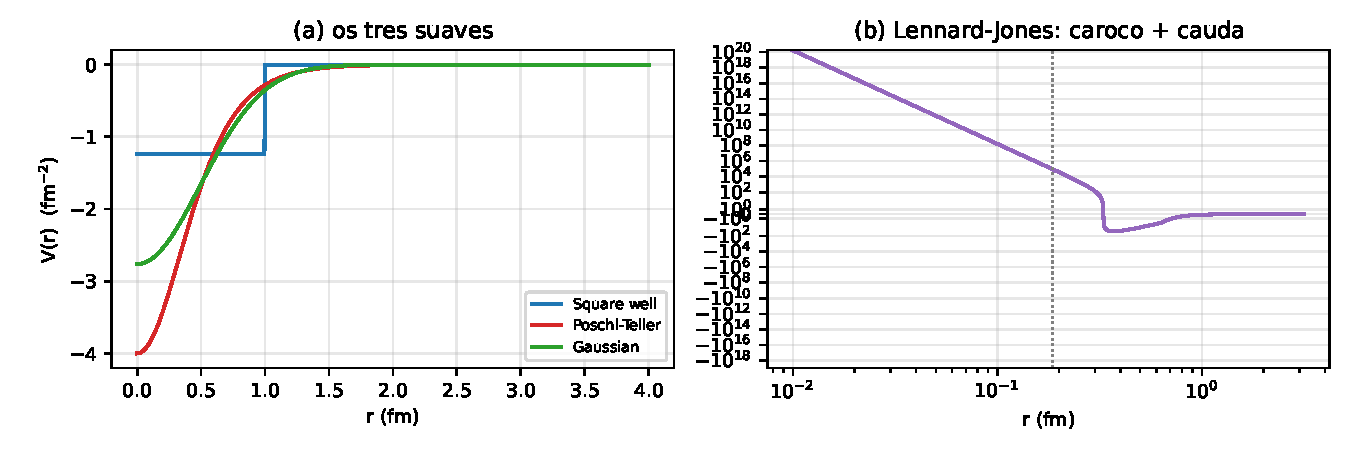
\includegraphics[width=\textwidth]{figuras/potenciais.pdf}
  \caption{Os quatro potenciais, todos sintonizados na unitariedade
  ($|a|\to\infty$). O Lennard-Jones precisa de eixos logarítmicos porque seu
  caroço chega a $10^{10}$ em unidades do código; a linha pontilhada marca
  \texttt{r\_min}, onde a integração começa.}
\end{figure}

\subsection{O alcance $R$, em forma fechada}

Cada classe precisa saber onde o potencial deixa de agir. Para o poço isso é
exato, $R = 1/\mu$. Para os outros três, o potencial nunca é zero de verdade ---
a gaussiana decai para sempre. Definimos então $R$ como o raio onde
$|V(R)| = \texttt{V\_ZERO}$, e resolvemos essa equação \emph{no papel}:

\begin{align}
  \text{Pöschl-Teller:}&\quad \frac{v\mu^2}{\cosh^2(\mu R)} = \varepsilon
    &&\Longrightarrow\quad R = \frac{1}{\mu}\,\mathrm{arccosh}\!\sqrt{\frac{v\mu^2}{\varepsilon}}\\
  \text{Gaussiano:}&\quad v\mu^2 e^{-\mu^2R^2} = \varepsilon
    &&\Longrightarrow\quad R = \frac{1}{\mu}\sqrt{\ln\frac{v\mu^2}{\varepsilon}}\\
  \text{Lennard-Jones (cauda):}&\quad \tfrac12 C_6/R^6 = \varepsilon
    &&\Longrightarrow\quad R = \left(\frac{C_6}{2\varepsilon}\right)^{1/6}\\
  \text{Lennard-Jones (caroço):}&\quad \tfrac12 C_{12}/r_{\min}^{12} = V_{\text{caroço}}
    &&\Longrightarrow\quad r_{\min} = \left(\frac{C_{12}}{2V_{\text{caroço}}}\right)^{1/12}
\end{align}

\pq{A versão anterior do código procurava esses raios numericamente, varrendo uma
grade global de 40\,000 pontos. Resolver no papel eliminou essa grade inteira,
uma função auxiliar, e deixou o resultado exato em vez de limitado pela
resolução da varredura.}

\begin{lstlisting}
class LennardJones:
    def __init__(self, C6, C12):
        self.C6 = C6
        self.C12 = C12
        self.r_min = (0.5 * C12 / V_CORE) ** (1.0 / 12.0)
        self.R     = (0.5 * C6  / V_ZERO) ** (1.0 /  6.0)

    def V(self, r):
        return 0.5 * (self.C12 / r ** 12 - self.C6 / r ** 6)
\end{lstlisting}

\subsection*{A armadilha do fator $\tfrac12$}

O $\tfrac12$ no Lennard-Jones é \textbf{convenção}, não física. Boa parte da
literatura escreve $C_{12}/r^{12}-C_6/r^6$ sem ele, o que desloca $C_6$ por um
fator dois --- e o resultado continua \emph{parecendo} certo. O artigo de
referência usa o $\tfrac12$, então o código usa também.

% ======================================================================
\section{Numerov: o integrador}

O método de Numerov resolve equações da forma $u'' = W(r)\,u$, que é exatamente
a nossa Eq.~\eqref{eq:radial} com $W = 2(V-E)$. A recursão é
\begin{equation}
  u_{i+1} = \frac{\bigl(12 - 10 f_i\bigr)u_i - f_{i-1}u_{i-1}}{f_{i+1}},
  \qquad f_i = 1 - \frac{h^2 W_i}{12}.
  \label{eq:numerov}
\end{equation}

\subsection*{De onde ela vem}

Expandindo $u_{i\pm1}$ em Taylor e somando,
\[
  u_{i+1} + u_{i-1} = 2u_i + h^2 u_i'' + \frac{h^4}{12}u_i^{(4)} + O(h^6).
\]
Um método de segunda ordem simplesmente joga fora o termo $h^4$. Numerov não:
como $u'' = Wu$, temos $u^{(4)} = (Wu)''$, e essa segunda derivada pode ser
aproximada pela \emph{mesma} diferença central, sem avaliar nada em pontos novos.
Substituindo e reagrupando sai a Eq.~\eqref{eq:numerov}.

\pq{É por isso que Numerov alcança ordem $h^4$ com o custo de um método de ordem
2. Ele nunca avalia $W$ fora dos pontos da grade. O preço é que a recursão usa
\emph{três} termos: cada ponto depende dos dois anteriores, então um erro
cometido no arranque viaja até o fim.}

\begin{lstlisting}
    f = 1.0 - h * h * W / 12.0
    for i in range(1, POINTS - 1):
        w[i + 1] = ((12.0 - 10.0 * f[i]) * w[i] - f[i - 1] * w[i - 1]) / f[i + 1]
\end{lstlisting}

% ======================================================================
\section{A grade logarítmica}
\label{sec:log}

\subsection{O problema}

Numerov exige $h\sqrt{|W|}\ll 1$ para representar a solução. Medindo isso nos
quatro potenciais em grade uniforme:

\begin{center}
\begin{tabular}{lrrl}
\toprule
\textbf{potencial} & $h$ (fm) & $\max|W|$ & $h\sqrt{|W|}$ \\
\midrule
poço esférico & 0{,}00103 & $8{,}3\times10^{-1}$ & 0{,}001 \\
Pöschl-Teller & 0{,}00851 & $2{,}1\times10^{0}$ & 0{,}012 \\
gaussiano     & 0{,}00401 & $1{,}6\times10^{0}$ & 0{,}005 \\
\textbf{Lennard-Jones} & 0{,}00626 & $\mathbf{2{,}0\times10^{5}}$ & \textbf{2{,}78} \\
\bottomrule
\end{tabular}
\end{center}

O Lennard-Jones tem um aperto sem saída: o caroço chega a $V=10^5$, logo
$\sqrt{2V}=447$ e o comprimento característico ali é $0{,}002$ fm; ao mesmo
tempo a cauda $1/r^6$ empurra $R$ para $125$ fm. \textbf{Nenhum passo uniforme
serve aos dois.}

A consequência foi medida, e é um erro de verdade: o $r_0$ do Lennard-Jones
\emph{derivava} conforme os pontos dobravam, em vez de convergir.

\begin{figure}[htbp]\centering
  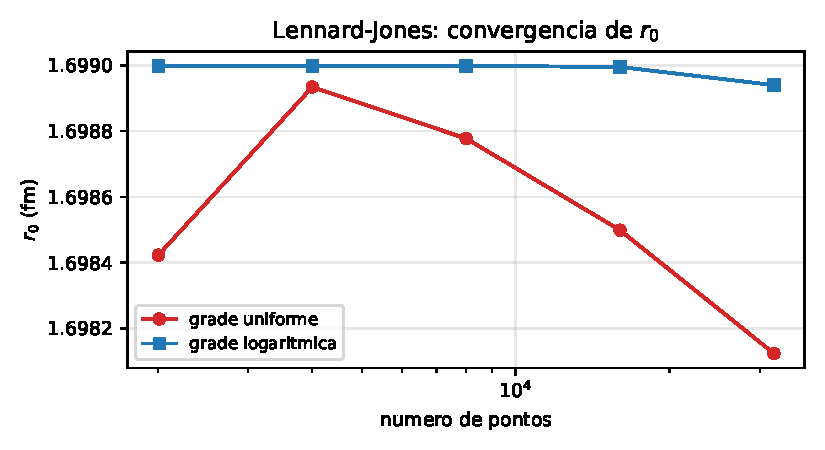
\includegraphics[width=0.72\textwidth]{figuras/convergencia.pdf}
  \caption{Teste de convergência. Em grade uniforme (vermelho) $r_0$ não
  estabiliza. Em grade logarítmica (azul) ele trava na quinta casa. Um resultado
  que muda quando você refina a grade não é um resultado.}
  \label{fig:conv}
\end{figure}

\begin{figure}[htbp]\centering
  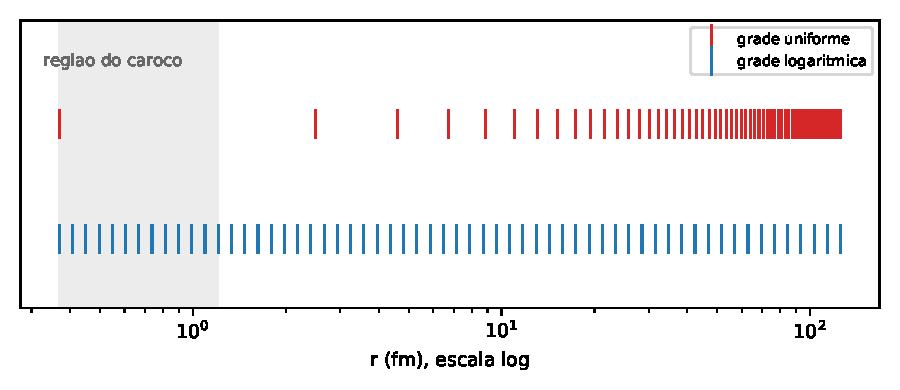
\includegraphics[width=0.8\textwidth]{figuras/grade.pdf}
  \caption{Distribuição dos pontos, mesmo número nos dois casos. A grade
  uniforme desperdiça quase tudo na cauda e deixa o caroço com meia dúzia de
  pontos; a logarítmica faz o contrário.}
\end{figure}

\subsection{A conta}

Fazendo $r = e^x$ e $u = e^{x/2}w(x)$, com $\dfrac{d}{dr} = e^{-x}\dfrac{d}{dx}$:
\begin{align}
  u' &= e^{-x}\frac{d}{dx}\bigl(e^{x/2}w\bigr)
      = e^{-x/2}\Bigl(\tfrac12 w + w'\Bigr),\\[4pt]
  u'' &= e^{-x}\frac{d}{dx}\Bigl[e^{-x/2}\bigl(\tfrac12 w + w'\bigr)\Bigr]
       = e^{-3x/2}\Bigl(w'' - \tfrac14 w\Bigr).
\end{align}
Levando na Eq.~\eqref{eq:radial}, $e^{-3x/2}(w''-\tfrac14 w) = 2(V-E)e^{x/2}w$, ou
\begin{equation}
  \boxed{\;w''(x) = \Bigl[\,2\bigl(V(e^x)-E\bigr)e^{2x} + \tfrac14\,\Bigr]\,w(x)\;}
  \label{eq:log}
\end{equation}

Dois fatos importam aqui. Primeiro, \textbf{apareceu um $\tfrac14$} que não
estava na equação original --- ele vem da substituição $u = e^{x/2}w$, não da
física. Segundo, e decisivo: a Eq.~\eqref{eq:log} continua na forma $w'' = W w$,
que é a \emph{única} coisa que Numerov exige. Por isso a recursão não muda uma
vírgula; só o que entra nela muda.

\pq{Trocar a variável independente é o recurso padrão quando o problema tem
duas escalas muito diferentes. Aqui elas diferem por cinco ordens de grandeza:
$0{,}002$ fm no caroço contra $125$ fm na cauda.}

\begin{lstlisting}
    r_start = pot.r_min if pot.r_min > 0.0 else pot.R * 1e-6
    x = np.linspace(math.log(r_start), math.log(pot.R), POINTS)
    h = x[1] - x[0]
    r = np.exp(x)
    W = 2.0 * (pot.V(r) - E) * r * r + 0.25
\end{lstlisting}

% ======================================================================
\section{Os dois arranques}

Numerov precisa de \emph{dois} valores iniciais, e o código escolhe entre dois
casos:

\begin{lstlisting}
    if pot.r_min > 0.0:
        w[1] = h * math.exp(x[0] / 2.0)      # caroco duro: u = 0, u' = 1
    else:
        w[0] = math.sqrt(r[0])               # origem regular: u ~ r
        w[1] = math.sqrt(r[1])
\end{lstlisting}

\textbf{Origem regular} (poço, Pöschl-Teller, gaussiano). Perto de $r=0$ com $V$
finito, a solução regular vale $u \simeq r$. Como $w = u\,e^{-x/2} = u/\sqrt{r}$,
isso dá $w \simeq \sqrt{r}$ --- que é exatamente o que o código escreve.

\textbf{Caroço duro} (Lennard-Jones). Ali $V$ explode e $u$ é exponencialmente
pequena; impomos $u(r_{\min}) = 0$ com inclinação unitária, e a mesma conversão
$w = u/\sqrt{r}$ dá $w_1 \simeq h\,e^{x_0/2}$.

\pq{Errar o arranque não é um detalhe local: pela recursão de três termos, o erro
se propaga por toda a integração. Um teste que fizemos: para o Lennard-Jones a
correção de ordem 4 no arranque, $u_1 = h + h^3W_0/6$, vale \emph{129\%} de $h$.
Ela não resolveu o problema daquela versão --- a causa era outra, a grade --- mas
mostra a escala do que está em jogo.}

% ======================================================================
\section{A derivada na borda}

Para colar a solução na fórmula analítica precisamos de $u(R)$ e $u'(R)$. O valor
sai direto; a derivada usa uma diferença lateral de cinco pontos:
\begin{equation}
  \frac{dw}{dx}\Big|_{R} \simeq
  \frac{25w_{N} - 48w_{N-1} + 36w_{N-2} - 16w_{N-3} + 3w_{N-4}}{12h}
  \;+\; O(h^4),
\end{equation}
e a volta para o raio físico vem da primeira linha da conta da Seção~\ref{sec:log}:
\begin{equation}
  \frac{du}{dr}\Big|_{R} = e^{-x_N/2}\Bigl(\tfrac12 w_N + \frac{dw}{dx}\Big|_R\Bigr).
\end{equation}

\pq{Duas razões para a fórmula lateral em vez de uma diferença central. Ela é de
ordem $h^4$, igual ao resto do método --- uma central seria $O(h^2)$ e
estragaria a ordem global. E ela usa \emph{só pontos internos}, então nunca
atravessa a descontinuidade do poço quadrado.}

\subsection*{O achado sobre a descontinuidade}

Se um passo de Numerov atravessa o salto do poço, o método assume que $W$ é suave
nos três pontos que usa --- e não é. Medimos a ordem de convergência:

\begin{center}
\begin{tabular}{rrl}
\toprule
$n$ & erro em $a$ & ordem medida \\
\midrule
2001  & $8{,}9\times10^{-4}$ & --- \\
4001  & $4{,}5\times10^{-4}$ & 1{,}00 \\
8001  & $2{,}2\times10^{-4}$ & 1{,}00 \\
16001 & $1{,}1\times10^{-4}$ & 1{,}00 \\
\bottomrule
\end{tabular}
\end{center}

Ordem exatamente 1, não 4. Com a grade terminando na borda e a derivada lateral,
o mesmo caso cai para $1{,}9\times10^{-10}$ --- \textbf{seis ordens de grandeza},
com o mesmo número de pontos.

% ======================================================================
\section{$a$ e $r_0$: o que o código mede}

\subsection{O comprimento de espalhamento}

Além de $R$ a solução é a reta $u = C(1 - r/a)$. Ela cruza o zero em $r=a$, e
conhecendo $u(R)$ e $u'(R)$ a reta está determinada:
\begin{equation}
  \boxed{\;a = R - \frac{u(R)}{u'(R)}\;}
\end{equation}

\pq{Isso é uma \emph{leitura exata}, não um ajuste. Não há mínimos quadrados,
não há extrapolação. A única fonte de erro é a integração até $R$.}

O código trata separadamente o caso $u'(R)=0$: a reta fica horizontal, nunca
cruza o zero, e $a = \infty$. Isso é unitariedade exata, não erro.

\begin{lstlisting}
    if slope == 0.0:
        a = math.inf
    else:
        a = pot.R - u[-1] / slope
\end{lstlisting}

\subsection{A normalização, e por que ela é necessária}

A Eq.~\eqref{eq:radial} é homogênea: se $u$ é solução, $Cu$ também é. O arranque
escolheu uma normalização arbitrária, então $u$ ainda não é comparável com nada.
Fixamos exigindo que ela encontre a reta na borda:
\begin{equation}
  u \;\longleftarrow\; u\,\frac{1 - R/a}{u(R)}
  \qquad\Longrightarrow\qquad u(R) = g_0(R), \quad g_0(r) \equiv 1 - \frac{r}{a}.
\end{equation}

\pq{Sem isso a integral do alcance efetivo não estaria definida --- ela compara
$u$ com $g_0$, e a comparação só faz sentido depois que as duas estão na mesma
escala.}

\subsection{O alcance efetivo}

\begin{equation}
  r_0 = 2\int_0^\infty \Bigl[g_0(r)^2 - u(r)^2\Bigr]dr .
  \label{eq:r0}
\end{equation}

O integrando mede \emph{o quanto a solução verdadeira se afasta da reta}, e por
isso é uma medida do tamanho do potencial. Fora do alcance $u = g_0$ e o
integrando é identicamente nulo, então a integral de fato termina em $R$.

Duas coisas no código:

\textbf{O fator $r$.} Na grade logarítmica $dr = r\,dx$, então a integral vira
$\int(\dots)\,r\,dx$. É de onde vem o \texttt{* r} na chamada do Simpson.

\textbf{O pedaço analítico.} A grade começa em $r_{\text{start}}$, não em zero.
O trecho $[0, r_{\text{start}}]$ entra na mão: ali $u$ é zero (dentro de um
caroço duro) ou proporcional a $r$, e nos dois casos a contribuição dela é
$O(r_{\text{start}}^3)$ enquanto a da reta é $O(r_{\text{start}})$. Sobra
\begin{equation}
  2\int_0^{s}g_0^2\,dr = 2\left(s - \frac{s^2}{a} + \frac{s^3}{3a^2}\right),
  \qquad s \equiv r_{\text{start}}.
\end{equation}

\pq{Esse termo existia só para o Lennard-Jones. Medindo, descobrimos que o poço
quadrado tinha um erro residual de $2{,}4\times10^{-6}$ em $r_0$ que era
exatamente esse pedaço faltando. Tornar o termo incondicional eliminou um
\texttt{if} \emph{e} melhorou a precisão em três ordens de grandeza --- foi para
$5{,}6\times10^{-12}$.}

\begin{lstlisting}
    r0 = 2.0 * simpson((line ** 2 - u ** 2) * r, x=x)
    s = r_start
    r0 = r0 + 2.0 * (s - s ** 2 / a + s ** 3 / (3.0 * a ** 2))
\end{lstlisting}

% ======================================================================
\section{Contar estados ligados sem procurá-los}

O código conta estados ligados contando \emph{zeros da solução de energia zero}.
Isso é o teorema de Levinson, e é surpreendente: a solução de espalhamento, em
$E=0$, sabe quantos estados ligados o potencial tem.

Há uma sutileza. Além da borda a solução é a reta $g_0 = 1 - r/a$, que cruza o
zero em $r = a$. Se $a > R$ esse zero é físico e conta. Se $a$ é efetivamente
infinito, o zero está no infinito e não conta --- daí o teste \texttt{R < a < 1e4}.

\begin{lstlisting}
    nodes = 0
    for i in range(1, POINTS - 1):
        if u[i] * u[i + 1] < 0.0:
            nodes = nodes + 1
    if pot.R < a < 1e4:
        nodes = nodes + 1
\end{lstlisting}

\pq{A contagem não é opcional. Duas soluções podem ter o mesmo $(a, r_0)$ e
números de nós diferentes --- e nesse caso \emph{não são o mesmo estado físico}.
Toda sintonia termina conferindo isso.}

\textbf{Um bug que passou por aqui:} o laço começa em \texttt{i = 1}, não em
\texttt{i = 0}. Como $u_0 = 0$ por construção, incluir o primeiro ponto contava
uma troca de sinal falsa e inflava a contagem em um para \emph{todo} potencial.

% ======================================================================
\section{O estado ligado}

Além da borda, com $E<0$, a solução tem que ser a exponencial que decai. Isso dá
a condição de casamento
\begin{equation}
  \boxed{\;g(E) \equiv u'(R) + \kappa\,u(R) = 0,\qquad \kappa = \sqrt{-2E}\;}
\end{equation}

\pq{Escrevemos a \emph{soma}, e não $u'/u + \kappa$, porque $u(R)$ pode passar
por zero --- o dêuteron tem um nó --- e a divisão inventaria um polo falso para
o localizador de raiz perseguir. Esse erro custou horas: com a razão, o dímero
de hélio dava resposta 100\% errada.}

\subsection*{Por que não há busca}

A fórmula de alcance finito já entrega a resposta com $\sim1\%$ de erro. Ela é o
palpite, e o \texttt{brentq} só refina dentro de $[1{,}8\,g,\;0{,}3\,g]$:

\begin{lstlisting}
    return brentq(gap, 1.8 * guess, 0.3 * guess, xtol=1e-15)
\end{lstlisting}

\pq{Uma versão anterior varria 120 energias numa grade logarítmica só para achar
onde a função trocava de sinal. Era desperdício: nós \emph{já tínhamos} a
resposta aproximada e a estávamos ignorando. Trocar a varredura pelo palpite
deixou o cálculo $3{,}5\times$ mais rápido \emph{e} mais exato. E há um bônus
conceitual: o fato de o intervalo funcionar sempre já é uma afirmação de que a
expansão de alcance efetivo é boa.}

% ======================================================================
\section{O problema inverso}

Dado um alvo $(a, r_0)$, achar os parâmetros. É um sistema $2\times2$ não-linear,
e $a$ tem \emph{polos}: ela salta de $+\infty$ para $-\infty$ toda vez que um
estado ligado novo aparece.

\subsection{A estrutura: dois laços aninhados}

\begin{center}
\begin{tabular}{ll}
\toprule
\texttt{tune} & laço externo: mexe na \textbf{escala} até $r_0$ bater \\
\quad\texttt{match\_a} & laço interno: mexe na \textbf{intensidade} até $1/a$ bater \\
\quad\quad\texttt{find\_root} & alarga o intervalo até trocar de sinal, então bissecta \\
\bottomrule
\end{tabular}
\end{center}

Cada laço resolve \emph{uma} equação em \emph{uma} variável. E dentro do laço
externo há uma função \texttt{r0\_error} que, a cada escala tentada, roda o laço
interno inteiro de novo --- é por isso que essa é a parte lenta do cálculo,
cerca de 35 dos 54 segundos totais.

\subsection*{A decisão que faz tudo funcionar: procurar raiz de $1/a$}

\pq{$a$ tem polos; $1/a$ é suave e cruza o zero. Bisseção \emph{morre} em cima de
um polo e prospera em cima de um zero. De brinde, unitariedade vira $1/a = 0$ e
não precisa de caso especial nenhum.}

\begin{lstlisting}
    if math.isinf(a_target):
        inv_a_target = 0.0
    else:
        inv_a_target = 1.0 / a_target
\end{lstlisting}

\subsection*{Por que não um Newton 2D}

As curvas de nível de $1/a$ e de $r_0$ no plano (intensidade, escala) são
\emph{quase paralelas} em boa parte do domínio. Um Newton nas duas equações de
uma vez encontraria uma jacobiana mal-condicionada exatamente ali, e daria passos
enormes na direção errada. Bisseção aninhada não tem como divergir depois que o
sinal está encapsulado --- mais lenta por iteração e muito mais confiável para um
código que outra pessoa vai rodar.

\subsection*{O retorno de seis valores}

\texttt{tune} devolve \texttt{(strength, scale, a, r0, nodes, ok)}. O último é
uma bandeira: ela é falsa se $r_0$ não convergiu \emph{ou} se a contagem de nós
não bateu com a exigida. Sem essa bandeira, uma sintonia que caiu no estado
errado passaria despercebida.

% ======================================================================
\section{Toda constante, uma por uma}

Nenhum número no código é chute. Esta tabela é a justificativa de cada um.

\begin{center}
\begin{tabular}{lll p{6.6cm}}
\toprule
\textbf{constante} & \textbf{valor} & \textbf{onde} & \textbf{justificativa} \\
\midrule
\texttt{V\_ZERO} & $10^{-12}$ & define $R$ &
  Abaixo disso o potencial é tratado como ausente. Testado: cortes de $10^{-8}$
  truncavam a cauda do Lennard-Jones e erravam $r_0$ em $0{,}16\%$; $10^{-12}$
  fecha em $0{,}004\%$. \\
\addlinespace
\texttt{V\_CORE} & $10^{5}$ & início do LJ &
  Onde a integração começa no caroço. Medido: em $10^{3}$ a física quebra
  ($r_0$ erra $0{,}2\%$); de $10^{4}$ para cima o resultado não muda mais. \\
\addlinespace
\texttt{POINTS} & 8001 & tamanho da grade &
  Erro total $=$ truncamento (cai com $n$) $+$ arredondamento (cresce com $n$);
  8001 está no mínimo. Os três suaves ficam em $10^{-11}$ e não se importam. O
  Lennard-Jones define o valor: passando de $\sim$8000 o $r_0$ dele \emph{piora}
  --- $3\times10^{-5}$ em 32001, $3\times10^{-4}$ em 64001. \\
\addlinespace
\texttt{r\_start} & $R\times10^{-6}$ & origem regular &
  Onde a grade logarítmica começa quando não há caroço. Não pode ser $0$ porque
  $\ln 0$ não existe. O trecho abaixo dele entra pela fórmula analítica. \\
\addlinespace
$[1{,}8g,\;0{,}3g]$ & --- & \texttt{brentq} &
  Intervalo em torno do palpite de alcance finito. Funciona nos dois sistemas
  testados; que funcione é um enunciado sobre a qualidade da expansão. \\
\addlinespace
$1{,}3$ & --- & \texttt{find\_root} &
  Fator de alargamento do intervalo, até 40 tentativas. Se não achar troca de
  sinal, levanta erro em vez de devolver lixo. \\
\addlinespace
$10^{-7}$, $10^{-6}$ & --- & tolerâncias &
  Convergência de $r_0$ no \texttt{tune} e nos testes. Medido: o \texttt{tune}
  acerta o alvo em $10^{-10}$, bem dentro delas. \\
\bottomrule
\end{tabular}
\end{center}

% ======================================================================
\section{Os dados tabelados}
\label{sec:dados}

Cinco dicionários, todos rastreáveis:

\begin{center}
\begin{tabular}{lp{10.4cm}}
\toprule
\texttt{TARGETS} & Tabela 2 do artigo: os três alvos, com o número de estados ligados exigido. \\
\texttt{PUBLISHED} & Tabelas 3 e 4: os parâmetros publicados. Servem de chute inicial \emph{e} de alvo de validação. \\
\texttt{SYSTEMS} & Tabela 1: dois sistemas reais, com energia medida. \\
\texttt{GUESS} & A solução do dêuteron, usada como ponto de partida para outros sistemas. \\
\texttt{SOURCES} & As três referências com DOI, mais a divergência \texttt{D1}. \\
\bottomrule
\end{tabular}
\end{center}

\subsection{A invariância de escala em \texttt{GUESS}}

O problema é invariante de escala: multiplicar todos os comprimentos por $L$ leva
$(a, r_0)\to(La, Lr_0)$. Então para atacar outro sistema basta reescalar o chute:
\begin{equation}
  \mu \;\to\; \frac{\mu}{L}, \qquad C_{12} \;\to\; C_{12}\,L^6 .
\end{equation}
O $L^6$ é porque $C_{12}$ multiplica $r^{-12}$, e $(Lr)^{-12} = L^{-12}r^{-12}$;
para $V$ escalar como $L^{-2}$ é preciso $C_{12}\to C_{12}L^{6}$... e o mesmo
raciocínio dá $C_6 \to C_6 L^{4}$.

\subsection{A constante que não está tabelada}

$\hbar^2/2\mu_{\text{red}}$ não aparece em tabela nenhuma. Nós a obtemos
invertendo a fórmula de alcance zero sobre o par publicado $(a, E_{zr})$:
\begin{equation}
  E_{zr} = -\frac{\hbar^2/2\mu_{\text{red}}}{a^2}
  \quad\Longrightarrow\quad
  \frac{\hbar^2}{2\mu_{\text{red}}} = -E_{zr}\,a^2 .
\end{equation}

\begin{center}
\begin{tabular}{lrrl}
\toprule
sistema & inferido & literatura & desvio \\
\midrule
dêuteron & $41{,}462$ MeV$\cdot$fm$^2$ & $41{,}47$ & $0{,}02\%$ \\
dímero de $^4$He & $12{,}095$ K$\cdot$\AA$^2$ & $12{,}12$ & $0{,}21\%$ \\
\bottomrule
\end{tabular}
\end{center}

\pq{Isso é um \textbf{teste}, não uma conveniência. Recuperar as duas constantes
conhecidas prova que a Tabela 1 do artigo é internamente consistente --- e, de
quebra, que o fator 2 da Eq.~\eqref{eq:conversao} está certo.}

\subsection*{A divergência \texttt{D1}}

Duas das doze sintonias desviam $2{,}7\%$ dos parâmetros publicados:
(nn, Lennard-Jones) e (dêuteron, Pöschl-Teller). A causa \emph{não} é numérica:
refinando a grade o desvio vai de $2{,}70\%$ para $2{,}69\%$. Os parâmetros
publicados no artigo produzem $r_0 = 2{,}71$ e $1{,}73$, enquanto a Tabela 2 do
\emph{mesmo} artigo lista os alvos como $2{,}70$ e $1{,}70$. Nós sintonizamos no
alvo e caímos em outro ponto --- corretamente.

\begin{quote}
\textbf{Regra geral:} discrepância que sobrevive ao refinamento nunca é numérica.
\end{quote}

% ======================================================================
\section{Os testes}

\texttt{test\_lab.py} tem oito verificações, e todas comparam com algo que o
código \textbf{não} calculou:

\begin{center}
\begin{tabular}{lp{8.4cm}}
\toprule
\textbf{verificação} & \textbf{âncora externa} \\
\midrule
$a$ do poço & Eq.~(80) do artigo, forma fechada \\
$r_0$ do poço & Eq.~(92) do artigo, forma fechada \\
$r_0/R = 1$ nos polos & previsão exata da Fig.~6 do artigo \\
estado ligado & condição analítica $k\cot(kR) = -\kappa$ \\
contagem de nós & Tabela 2, nos 12 casos \\
sintonia & Tabelas 3 e 4, nos 12 casos \\
constantes inferidas & $41{,}47$ e $12{,}12$ da literatura \\
convergência da grade & dividir os pontos pela metade não pode mudar nada \\
\bottomrule
\end{tabular}
\end{center}

\pq{Nenhum teste diz ``igual à última vez''. Um teste desses só provaria que o
código é consistente com os próprios erros.}

O último foi o que \emph{achou} o bug da grade uniforme. Ele divide os pontos
pela metade em vez de dobrar, e isso é deliberado: como o erro total tem um
mínimo, a pergunta útil é ``já convergimos vindo de baixo?'' e não ``o que
acontece fundo na região de arredondamento?''.

% ======================================================================
\section{Autópsia: os erros que cometemos}
\label{sec:autopsia}

Esta seção existe porque a causa de um erro costuma valer mais que o resultado.

\subsection*{1. Numerov caindo de ordem 4 para ordem 1}
\textbf{Sintoma:} o poço quadrado convergia devagar demais.
\textbf{Causa:} um passo atravessava a descontinuidade; Numerov supõe $W$ suave
nos três pontos que usa. \textbf{Conserto:} a grade termina exatamente na borda
e a derivada usa só pontos internos. \textbf{Ganho:} seis ordens de grandeza.

\subsection*{2. O $r_0$ do Lennard-Jones derivando}
\textbf{Sintoma:} $1{,}74257 \to 1{,}74215 \to 1{,}74165$ conforme os pontos
dobravam. \textbf{Diagnóstico:} descartamos duas hipóteses erradas antes de
achar a certa --- não era a cauda (truncar em 30 fm mantinha a deriva) e não era
o arranque (corrigir para ordem 4 não mudou nada). Era $h\sqrt{|W|} = 2{,}78$ no
caroço. \textbf{Conserto:} grade logarítmica. \textbf{Confirmação:} o valor novo
bate com um método independente (integrador adaptativo) em 7 dígitos.

\subsection*{3. Casar a solução dentro do poço}
\textbf{Sintoma:} a energia do poço saía $0{,}44\%$ errada.
\textbf{Causa:} o casamento usava o \emph{último} ponto onde o potencial ainda
agia --- que, no poço, é dentro, onde $V\neq0$. \textbf{Conserto:} casar do lado
de fora.

\subsection*{4. O nó falso na origem}
\textbf{Sintoma:} todo potencial reportava um estado ligado a mais.
\textbf{Causa:} $u_0 = 0$ por construção contava como troca de sinal.
\textbf{Conserto:} começar o laço em \texttt{i = 1}.

\subsection*{5. O termo interno que só existia para o LJ}
\textbf{Sintoma:} erro residual de $2{,}4\times10^{-6}$ em $r_0$ do poço.
\textbf{Causa:} a grade logarítmica não cobre $[0, r_{\text{start}}]$, e o termo
analítico estava dentro de um \texttt{if}. \textbf{Conserto:} torná-lo
incondicional --- um \texttt{if} a menos e três ordens de grandeza a mais.

\subsection*{6. O escape de \LaTeX{} incompleto}
\textbf{Sintoma:} ``Missing \$ inserted'' numa tabela visualmente perfeita.
\textbf{Causa:} o mapa de caracteres não incluía \verb|^|, e a tabela continha
\verb|pi^2/8|. \textbf{Lição:} erro de \LaTeX{} raramente está onde ele reclama.

% ======================================================================
\section{Resultados}

\begin{figure}[htbp]\centering
  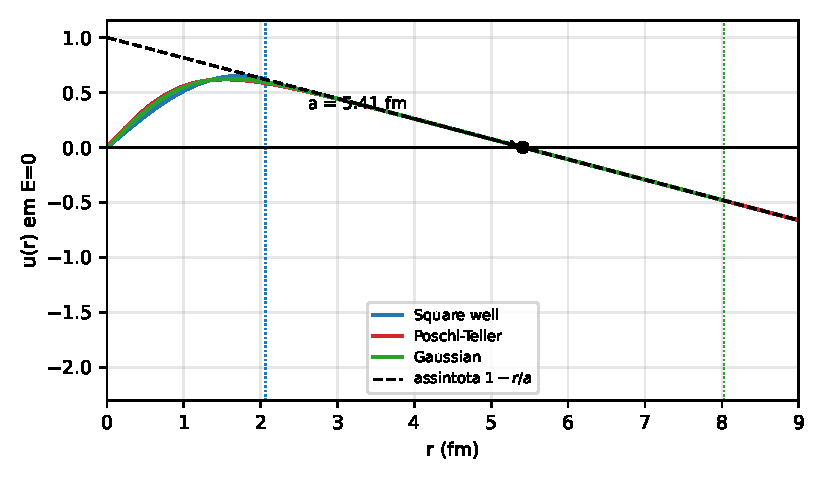
\includegraphics[width=0.72\textwidth]{figuras/ondas.pdf}
  \caption{\textbf{A figura que responde a pergunta.} Três potenciais
  sintonizados no mesmo $(a, r_0)$ do dêuteron: as funções de onda são
  \emph{idênticas fora} do alcance e \emph{completamente diferentes dentro}. As
  pontilhadas marcam onde cada potencial termina. Tudo o que um experimento de
  baixa energia enxerga mora do lado de fora.}
\end{figure}

\begin{figure}[htbp]\centering
  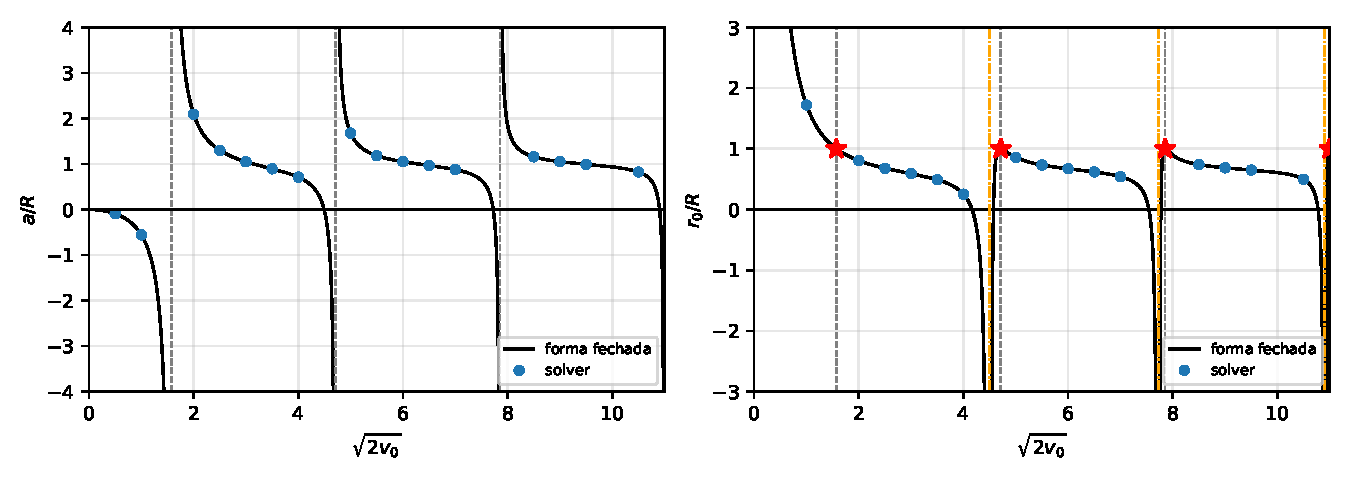
\includegraphics[width=\textwidth]{figuras/artigo56.pdf}
  \caption{Reprodução das Figs.~5 e 6 do artigo. Esquerda: $a/R$ diverge em
  $\sqrt{2v_0} = \pi/2 + n\pi$, onde nasce um estado ligado novo. Direita: em
  cada um desses pontos $r_0/R = 1$ \emph{exatamente} (estrelas vermelhas) --- o
  alcance efetivo iguala o alcance do potencial. As linhas laranja marcam a
  \emph{outra} família de singularidades, as raízes de $\tan x = x$, onde $a=0$
  e é $r_0$ que diverge.}
\end{figure}

\subsection{Energias de ligação}

\begin{center}
\begin{tabular}{lrr rr}
\toprule
& \multicolumn{2}{c}{\textbf{dêuteron} ($|a|/r_0 = 3{,}1$)}
& \multicolumn{2}{c}{\textbf{dímero de $^4$He} ($|a|/r_0 = 11{,}3$)} \\
\cmidrule(lr){2-3}\cmidrule(lr){4-5}
método & $E$ (MeV) & desvio & $E$ (K) & desvio \\
\midrule
experimento        & $-2{,}224$ & --- & $-1{,}620\times10^{-3}$ & --- \\
alcance zero       & $-1{,}416$ & $-36{,}3\%$ & $-1{,}480\times10^{-3}$ & $-8{,}6\%$ \\
alcance finito     & $-2{,}223$ & $-0{,}05\%$ & $-1{,}628\times10^{-3}$ & $+0{,}47\%$ \\
\midrule
poço esférico      & $-2{,}204$ & $-0{,}91\%$ & $-1{,}627\times10^{-3}$ & $+0{,}46\%$ \\
Pöschl-Teller      & $-2{,}227$ & $+0{,}11\%$ & $-1{,}628\times10^{-3}$ & $+0{,}47\%$ \\
gaussiano          & $-2{,}214$ & $-0{,}47\%$ & $-1{,}627\times10^{-3}$ & $+0{,}46\%$ \\
Lennard-Jones      & $-2{,}203$ & $-0{,}92\%$ & --- & --- \\
\bottomrule
\end{tabular}
\end{center}

\subsection*{Como ler}

A fórmula de alcance zero erra $36\%$ no dêuteron e $8{,}6\%$ no hélio. O que
separa os dois é a razão $|a|/r_0$: vale $3{,}1$ e $11{,}3$. \textbf{O dêuteron,
que é o exemplo didático clássico de estado ligado raso, reprova no critério
usual de universalidade $|a|/r_0 > 10$.} Incluir $r_0$ derruba os dois para menos
de $1\%$. E o espalhamento residual de $\sim1\%$ \emph{entre} os potenciais é a
dependência de forma --- os termos $O(k^4)$, a única coisa que ainda distingue um
poço quadrado de um Lennard-Jones depois que $a$ e $r_0$ foram fixados.

\subsection{Exatidão alcançada}

\begin{center}
\begin{tabular}{lr}
\toprule
verificação & erro \\
\midrule
$a$ do poço contra a Eq.~(80) & $1{,}9\times10^{-10}$ \\
$r_0$ do poço contra a Eq.~(92) & $5{,}6\times10^{-12}$ \\
estado ligado contra $k\cot(kR)=-\kappa$ & $3{,}4\times10^{-10}$ \\
$r_0/R$ nos quatro polos & $1{,}0000000000$ \\
solver contra formas fechadas (16 pontos) & $8{,}4\times10^{-9}$ \\
sintonia acertando o alvo & $10^{-10}$ \\
\bottomrule
\end{tabular}
\end{center}

% ======================================================================
\section{O que falta}

\textbf{Sem barras de erro.} Nenhum número aqui tem incerteza de discretização
estimada. O módulo \texttt{src/comum/incerteza.py} tem extrapolação de Richardson
e portões de validade prontos para isso.

\textbf{Lennard-Jones no hélio.} Com $a = 90$ \AA{} a cauda só morre depois de
milhares de \AA. Fica de fora da tabela.

\textbf{$r_0$ do Lennard-Jones.} Confiável até $\sim10^{-6}$, limitado por
arredondamento, não por truncamento.

\textbf{Só onda-$s$.} Válido enquanto $kR \ll 1$.

\subsection*{O que este código já entrega}

Um motor que, dado um alvo $(a, r_0)$, devolve os parâmetros de qualquer um dos
quatro potenciais e a energia de ligação correspondente, com exatidão verificada
contra formas fechadas. É a peça de base: qualquer cálculo de muitos corpos que
venha depois precisa de um potencial de dois corpos ancorado em $(a, r_0)$
conhecidos, e é exatamente isso que ele produz.

% ======================================================================
\begin{thebibliography}{9}
\bibitem{rbef}
  M.~Macêdo-Lima e L.~Madeira,
  \emph{Scattering length and effective range of microscopic two-body potentials},
  Rev.\ Bras.\ Ensino Fís.\ \textbf{45}, e20230079 (2023).
  \href{https://doi.org/10.1590/1806-9126-RBEF-2023-0079}{doi:10.1590/1806-9126-RBEF-2023-0079}

\bibitem{hack}
  R.~W.~Hackenburg,
  \emph{Low-energy neutron-proton effective range parameters},
  Phys.\ Rev.\ C \textbf{73}, 044002 (2006).
  \href{https://doi.org/10.1103/PhysRevC.73.044002}{doi:10.1103/PhysRevC.73.044002}

\bibitem{cencek}
  W.~Cencek \emph{et al.},
  \emph{Effects of adiabatic, relativistic, and QED corrections on the pair
  potential of helium},
  J.\ Chem.\ Phys.\ \textbf{136}, 224303 (2012).
  \href{https://doi.org/10.1063/1.4712218}{doi:10.1063/1.4712218}
\end{thebibliography}


% ======================================================================
\appendix
\section{As três funções, na íntegra}

Esta seção traz o corpo completo das funções centrais, para que nenhuma linha
fique sem explicação. Os comentários numerados remetem às notas logo abaixo de
cada bloco.

\subsection{\texttt{numerov} --- o integrador}

\begin{lstlisting}
def numerov(pot, E):
    r_start = pot.r_min if pot.r_min > 0.0 else pot.R * 1e-6          # (1)

    x = np.linspace(math.log(r_start), math.log(pot.R), POINTS)       # (2)
    h = x[1] - x[0]
    r = np.exp(x)
    W = 2.0 * (pot.V(r) - E) * r * r + 0.25                           # (3)
    f = 1.0 - h * h * W / 12.0                                        # (4)

    w = np.zeros(POINTS)
    if pot.r_min > 0.0:
        w[1] = h * math.exp(x[0] / 2.0)                               # (5)
    else:
        w[0] = math.sqrt(r[0])                                        # (6)
        w[1] = math.sqrt(r[1])
    for i in range(1, POINTS - 1):
        w[i + 1] = ((12.0 - 10.0*f[i]) * w[i] - f[i-1]*w[i-1]) / f[i+1]   # (7)

    u = np.exp(x / 2.0) * w                                           # (8)

    dwdx = (25.0*w[-1] - 48.0*w[-2] + 36.0*w[-3]
            - 16.0*w[-4] + 3.0*w[-5]) / (12.0 * h)                    # (9)
    slope = math.exp(-x[-1] / 2.0) * (0.5 * w[-1] + dwdx)             # (10)

    return r, u, x, h, slope, r_start
\end{lstlisting}

\begin{enumerate}\setlength\itemsep{1pt}
\item Onde começar. Fora do caroço se houver um; senão perto da origem, porque
      $\ln 0$ não existe. O trecho pulado entra pela fórmula analítica.
\item A grade é uniforme em $x=\ln r$, e termina \emph{exatamente} em $\ln R$.
\item O potencial efetivo da Eq.~\eqref{eq:log}. O $r^2$ vem do $e^{2x}$; o
      $0{,}25$ é o $\tfrac14$ que a substituição gerou.
\item O $f$ de Numerov. Note que ele é um \emph{vetor}: calculado de uma vez
      para toda a grade, antes do laço.
\item Arranque com caroço: $u=0$, $u'=1$, convertido por $w=u/\sqrt{r}$.
\item Arranque regular: $u\simeq r$, logo $w\simeq\sqrt{r}$. Precisa dos
      \emph{dois} primeiros pontos porque a recursão é de três termos.
\item A recursão. É a única linha que de fato integra a equação.
\item Volta de $w$ para $u$. A partir daqui tudo está em unidades físicas.
\item Derivada lateral de cinco pontos, ordem $h^4$, só com pontos internos.
\item Conversão da derivada para o raio: $du/dr = e^{-x/2}(w/2 + dw/dx)$.
\end{enumerate}

\subsection{\texttt{scattering} --- as três leituras}

\begin{lstlisting}
def scattering(pot):
    r, u, x, h, slope, r_start = numerov(pot, 0.0)                    # (1)

    if slope == 0.0:
        a = math.inf                                                  # (2)
    else:
        a = pot.R - u[-1] / slope

    u = u * (1.0 - pot.R / a) / u[-1]                                 # (3)
    line = 1.0 - r / a

    r0 = 2.0 * simpson((line ** 2 - u ** 2) * r, x=x)                 # (4)
    s = r_start
    r0 = r0 + 2.0 * (s - s**2 / a + s**3 / (3.0 * a**2))              # (5)

    nodes = 0
    for i in range(1, POINTS - 1):                                    # (6)
        if u[i] * u[i + 1] < 0.0:
            nodes = nodes + 1
    if pot.R < a < 1e4:
        nodes = nodes + 1                                             # (7)

    return a, r0, nodes
\end{lstlisting}

\begin{enumerate}\setlength\itemsep{1pt}
\item Energia zero: é o único caso em que a solução externa é uma reta.
\item Reta horizontal significa unitariedade exata, e $a=\infty$ é a resposta
      certa --- não um erro a ser evitado.
\item A normalização. Sem ela a integral seguinte não estaria definida, porque
      a equação é homogênea.
\item A integral da Eq.~\eqref{eq:r0}. O \texttt{* r} é o jacobiano $dr = r\,dx$.
\item O pedaço $[0, r_{\text{start}}]$, feito no papel.
\item O laço começa em 1: incluir $u_0=0$ contaria um nó falso.
\item O nó exterior, em $r=a$, que só existe se $a$ for finito e maior que $R$.
\end{enumerate}

\subsection{\texttt{tune} --- o problema inverso}

\begin{lstlisting}
def tune(name, a_target, r0_target, strength, scale, nodes_target=None):
    if math.isinf(a_target):
        inv_a_target = 0.0                                            # (1)
    else:
        inv_a_target = 1.0 / a_target

    for step in range(25):                                            # (2)
        strength = match_a(name, scale, strength, inv_a_target)       # (3)
        a, r0, nodes = scattering(POTENTIALS[name](strength, scale))
        if abs(r0 - r0_target) < 1e-7:
            break

        def r0_error(trial_scale):                                    # (4)
            s = match_a(name, trial_scale, strength, inv_a_target)
            a2, r02, n2 = scattering(POTENTIALS[name](s, trial_scale))
            return r02 - r0_target

        scale = find_root(r0_error, scale)

    strength = match_a(name, scale, strength, inv_a_target)           # (5)
    a, r0, nodes = scattering(POTENTIALS[name](strength, scale))

    ok = abs(r0 - r0_target) < 1e-6
    if nodes_target is not None and nodes != nodes_target:
        ok = False                                                    # (6)

    return strength, scale, a, r0, nodes, ok
\end{lstlisting}

\begin{enumerate}\setlength\itemsep{1pt}
\item Unitariedade sem caso especial: $a=\infty$ é simplesmente $1/a=0$.
\item Vinte e cinco tentativas no máximo. Se sair antes, é porque convergiu.
\item Laço interno: acerta a intensidade para $1/a$ bater, com a escala fixa.
\item Esta função aninhada é o custo do algoritmo: a cada escala tentada, ela
      roda o laço interno \emph{inteiro} outra vez.
\item Um último acerto da intensidade, porque a escala mudou por último.
\item A bandeira \texttt{ok}. Sem ela, uma sintonia que caiu no estado errado
      passaria despercebida.
\end{enumerate}

\section{Os dados, com os valores}

\subsection*{\texttt{TARGETS} --- Tabela 2 do artigo}
\begin{center}
\begin{tabular}{lrrc}
\toprule
caso & $a$ (fm) & $r_0$ (fm) & estados ligados \\
\midrule
\texttt{nn} (nêutron-nêutron) & $-18{,}5$ & $2{,}7$ & 0 \\
\texttt{unitarity} & $\infty$ & $1{,}0$ & 0 \\
\texttt{deuteron} & $5{,}4$ & $1{,}7$ & 1 \\
\bottomrule
\end{tabular}
\end{center}

\subsection*{\texttt{PUBLISHED} --- Tabelas 3 e 4, e o que a sintonia devolve}
\begin{center}
\footnotesize
\begin{tabular}{llrrrrr}
\toprule
caso & potencial & $p_1$ obtido & $p_1$ publicado & $p_2$ obtido & $p_2$ publicado & desvio \\
\midrule
nn & poço          & 1{,}109228 & 1{,}1096 & 0{,}391087 & 0{,}3918 & 0{,}18\% \\
nn & Pöschl-Teller & 0{,}907086 & 0{,}9071 & 0{,}799622 & 0{,}7991 & 0{,}07\% \\
nn & gaussiano     & 1{,}211903 & 1{,}2121 & 0{,}567906 & 0{,}5672 & 0{,}12\% \\
nn & Lennard-Jones & 9{,}760657 & 9{,}8667 & 3{,}005560 & 3{,}0884 & \textbf{2{,}68\%} \\
\addlinespace
unit. & poço          & 1{,}233701 & 1{,}2337 & 1{,}000000 & 1{,}0000 & 0{,}00\% \\
unit. & Pöschl-Teller & 1{,}000000 & 1{,}0000 & 2{,}000000 & 2{,}0000 & 0{,}00\% \\
unit. & gaussiano     & 1{,}342002 & 1{,}3420 & 1{,}435224 & 1{,}4349 & 0{,}02\% \\
unit. & Lennard-Jones & 0{,}264625 & 0{,}2646 & 0{,}000341 & 0{,}00034 & 0{,}00\% \\
\addlinespace
dêut. & poço          & 1{,}758644 & 1{,}7575 & 0{,}499215 & 0{,}5000 & 0{,}16\% \\
dêut. & Pöschl-Teller & 1{,}423895 & 1{,}4388 & 0{,}886001 & 0{,}8631 & \textbf{2{,}65\%} \\
dêut. & gaussiano     & 1{,}910904 & 1{,}9102 & 0{,}674817 & 0{,}6754 & 0{,}09\% \\
dêut. & Lennard-Jones & 6{,}846862 & 6{,}8147 & 0{,}915045 & 0{,}9049 & 1{,}13\% \\
\bottomrule
\end{tabular}
\end{center}

\noindent
As duas linhas em negrito são a divergência \texttt{D1}: os parâmetros
publicados alcançam $r_0 = 2{,}71$ e $1{,}73$, enquanto a Tabela~2 do mesmo
artigo pede $2{,}70$ e $1{,}70$. Refinar a grade não move esses desvios.

\subsection*{\texttt{SYSTEMS} --- Tabela 1, os dois sistemas reais}
\begin{center}
\begin{tabular}{lrrrr}
\toprule
sistema & $a$ & $r_0$ & $E$ medida & $\hbar^2/2\mu$ inferido \\
\midrule
dêuteron & $5{,}4112$ fm & $1{,}7436$ fm & $-2{,}224$ MeV & $41{,}462$ MeV$\cdot$fm$^2$ \\
dímero de $^4$He & $90{,}4$ \AA & $8{,}0$ \AA & $-1{,}62$ mK & $12{,}095$ K$\cdot$\AA$^2$ \\
\bottomrule
\end{tabular}
\end{center}

\end{document}
